\section{Tracking}
\label{section: tracking}

The LHCb tracking system consists of the VELO; the Tracker Turicensis (TT) and the T1, T2 and T3 detectors (collectively called the T-stations), see figure \ref{fig: lhcb_schematic}. 

\subsection{Tracker Turicensis (TT)}
The Tracker Turicensis is located before the magnet and after the VELO detector. In addition to charged particles produced in the VELO detector the location of the TT allows it to provide tracking information for charged particles produced from the decay of long lived neutral particles such as the $K_S^0$ which may not decay in the VELO detector. It also provides tracking information for charged particles with low momentum which may not reach the T-stations downstream of the magnet due to the bending of then magnet.

The TT is a silicon micro strip detector with height of 1.5 m and width of 1.3 m, covering the full angular acceptance of the LHCb detector. It consists of 4 layers, the first and last are made up of vertical strips, the second and third inner layers have strips which have been rotated by 5 $^\circ$ and -5 $^\circ$ stereo angle to provide the transverse position of particles.

\begin{figure}
	\centering
	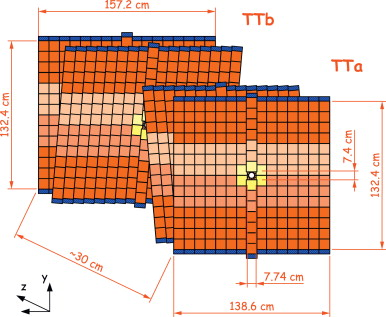
\includegraphics{Chapters/detector/images/tracker_turicensis_schematic.jpg}
	\caption{Layout of the 4 stations which constitutes the Tracker Turicensis}
	\label{fig: trigger turicensis schematic}
\end{figure}

\subsection{T-Stations T1, T2 and T3}

The T-stations are positioned after the magnet (see figure \ref{fig: lhcb_schematic}). Together with the tracking detectors upstream of the magnet the trajectory of charged particles through the magnetic field can be measured. The Lorentz force causes the trajectory of charged particles to bend as it traverses the magnetic field; from this the momentum of the track can be measured.

\subsection{Track Reconstruction}
\label{subsection: tracking, track reconstruction}

Track reconstruction at the LHCb detector is carried out via several different tracking strategies; generally these involve reconstructing tracks at the sub-detector level called track segments. For example tracks may be reconstructed purely from hits in the VELO sub-detector, these are known as VELO tracks. Similarly tracks may be reconstructed only from hits in the T-stations positioned downstream of the LHCb magnet. These segments may then be combined with hits in other trackers or other track segments to give a more detailed description of the corresponding particle. For example a VELO track segment may be combined with hits from the TT tracker to give an Upstream track, similarly a T-station track segment may also be combined with hits in the TT tracker to give a Downstream track. The possible track types are outline in figure \ref{fig: track types} and a more detailed description of each of the strategies can be found at \cite{lhcb_track_strategies}.

\begin{figure}[h]
	\centering
	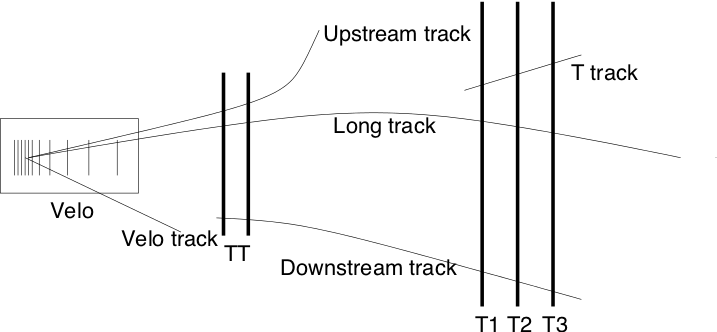
\includegraphics[width=0.8\textwidth]{/Users/admin/Dropbox/PhD/Thesis/Chapters/detector/tracking/images/tracktypes.png}
	\caption{LHCb Track Types}
	\label{fig: track types}
\end{figure}
